\documentclass[12pt]{article}

\usepackage{amsmath}
\usepackage{amsfonts}
\usepackage{hyperref}
\usepackage{enumitem}
\usepackage{graphicx}
\usepackage{abstract}
\usepackage{geometry}

% page settings
\geometry{a4paper, margin=1in} % sets A4 paper with 1-inch margins

% Title Page
\title{\textbf{Discrete Bulk Reconstruction Problem} \\ \large Compiled Research}
\author{Piper Jeffries \\ Missouri S\&T \\ \texttt{pejbvy@umsystem.edu}}
\date{\today}

\begin{document}

\maketitle

%%%%%%%%%%%%%%% ABSTRACT %%%%%%%%%%%%%%%%%%%%%%%%%%%%%%
\begin{abstract}
    The \textbf{Discrete Bulk Reconstruction Problem (DBRP)} models the entanglement structure of quantum systems using discrete graphs. It is rooted in the Anti-de Sitter / Conformal Field Theory (AdS/CFT) correspondence, which connects a gravitational theory in AdS space (the bulk) to its quantum field theory on its boundary (the CFT).
    While this describes a universe different from our own, it offers valuable insights into quantum gravity and spacetime emergence. 
    \\
    \indent Instead of using traditional approaches that rely on continous AdS space, DBRP models the bulk as a graph, where nodes correspond to regions of space and edge weights encode entanglement connectivity.
    In this framework, geodesics in AdS are approximated by min-cuts in the graph, and the Ryu-Takayanagi (RT) formula determines minimal surfaces in the bulk, allowing for bulk geometry reconstruction from boundary entanglement.
    \\
   \indent DBRP leverages tensory networks and holography to provide a discrete approach to understanding spacetime, quantum entanglement, and information flow.
    DBRP could provide profound insight in quantum gravity, improved quantum error correction, and practical quantum computing applications.
\end{abstract}

\newpage 
\tableofcontents
\newpage

%%%%%%%%%%%%%% INTRO %%%%%%%%%%%%%%%%%%%%%%%%%%
\section{Introduction}
    \hspace{0.5cm} DBRP aims to reconstruct spacetime (the bulk) from the entanglement structure of quantum systems. This structure is defined by the collection of entanglement entropies of its subsystems, which quantify how much information a given region of the system contains. More precisely, entanglement entropy measures how strongly a subsystem is correlated with the rest of the system.
    \\
    \indent A key motivation for DBRP comes from the AdS/CFT correspondence, first proposed by Juan Maldacena in 1997. This duality suggests that a (d + 1)-dimensional anti-de Sitter (AdS) space, which includes quantum gravity, is fully encoded by a d-dimensional conformal field theory (CFT) on its boundary. Because the CFT is non-gravitational, computations are easier, making this framework a powerful tool for understanding quantum gravity.
    \\
    \indent By leveraging insights from AdS/CFT, DBRP offers a discrete, graph-based approach to bulk reconstruction, which allows for a new perspective on how spacetime emerges from entanglement, with potential applications in both holography and quantum information theory.

%%%%%%%%%%%%%%%% 2 %%%%%%%%%%%%%%%%%%%%%%%%%%%%
\section{Explanation of "Universe"}
    \subsection{AdS (Anti-de Sitter) Space $\Rightarrow$ The Bulk}
        \begin{itemize}
            \item The \textbf{bulk} represents a higher-dimensional space in the AdS/CFT framework.  
            \item A \textbf{surface} is a geometric object within AdS space that plays a crucial role in holography.  
            \item The \textbf{minimal area} surface, also known as the RT surface in AdS/CFT, spans the boundary subregion and has the smallest possible area.  
            \item Since direct calculations in the bulk are challenging due to quantum gravity, computations are instead performed on the CFT boundary.  
        \end{itemize}

    \subsection{CFT (Conformal Field Theory) Space $\Rightarrow$ The Boundary}
        \begin{itemize}
            \item The \textbf{boundary} represents a lower-dimensional space that forms the "edge" or "boundary" of the AdS bulk.
            \item The \textbf{CFT} is a non-gravitational theory that lives on the boundary of the AdS spacetime.
            \item The information of the boundary is encoded in the bulk. The bulk and boundary are related by the holographic principle.
        \end{itemize}

        %% Photo of AdS/ CFT space 
        \begin{figure}[htbp]
            \centering
            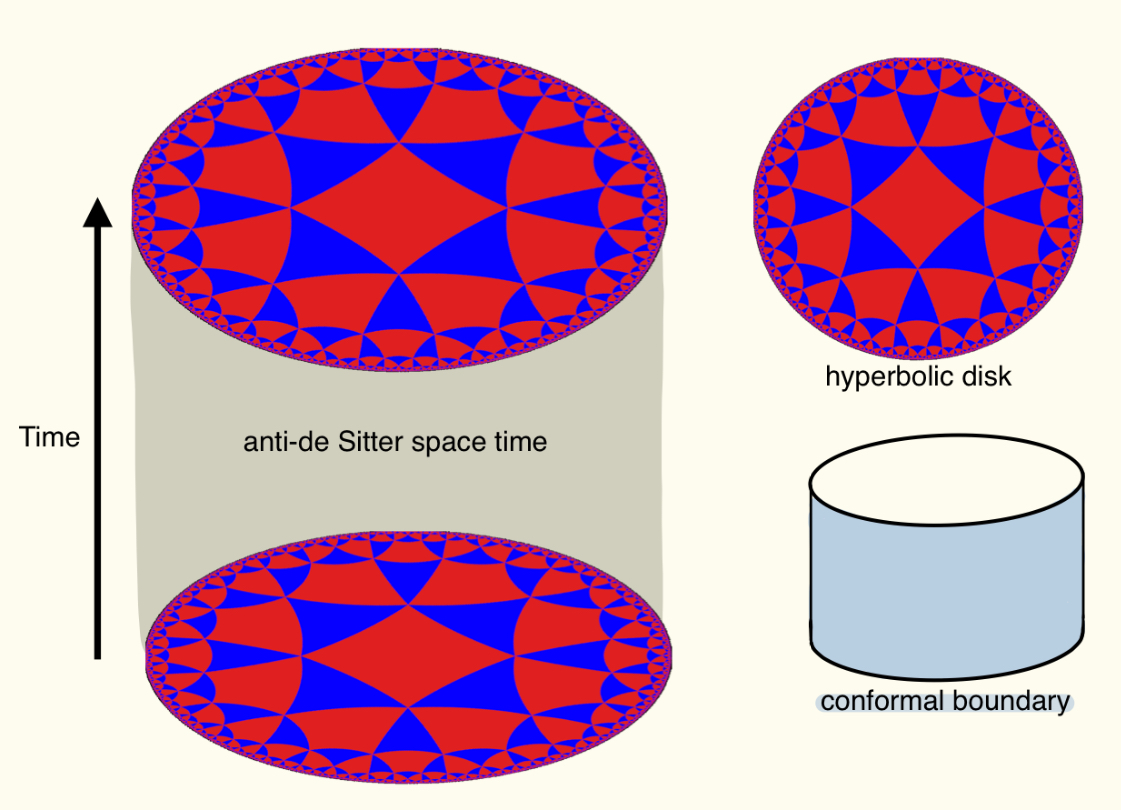
\includegraphics[width=0.8\textwidth]{ads_cft.jpeg}  
            \caption{This illustration shows the AdS/CFT spacetime. A geodesic is a straight line across the hyperbolic disk, which is the shortest path between points. In the context of anti-de Sitter spacetime, a geodesic represents the path that a particle follows when only affected by gravity.}  
            \label{fig:AdS/CFT space}  
        \end{figure}

        \newpage
        When dealing with a 5-dimensional AdS bulk, the boundary is typically 4-dimensional, and the CFT lives on this 4-dimensional boundary. This illustrates the idea that the boundary is one dimension less than the bulk. The boundary is where we will perform our computations, as it is easier to compute without gravity. Using the CFT, we can reconstruct the gravitational dynamics of the AdS bulk, which corresponds to the geodesics of the hyperbolic disk. Geodesics in AdS space are curved, unlike straight lines in flat geometry, even though they represent the shortest path between points. This curvature reflects the negative curvature of AdS space and the effects of gravity.

        These gravitational dynamics come from the entanglement entropy in the CFT. In AdS/CFT, the entanglement entropy on the boundary CFT encodes information about the geometry of the bulk. Given a CFT state, we can determine the corresponding spacetime that the CFT describes, including its geometry and gravitational dynamics. This allows us to extract bulk information, such as spacetime curvature, directly from the boundary CFT state. Thus, we can use the CFT to reconstruct the AdS bulk.

        \textbf{AdS/CFT correspondence} means that the gravitational theory in the bulk is equivalent to the non-gravitational CFT on the boundary. In other words, the two theories describe the same physics but from different perspectives: one is a gravitational theory, and the other is a quantum field theory without gravity. This is an extraordinary idea because it suggests that gravity can be understood in terms of a simpler quantum field theory on the boundary, offering insights into quantum gravity through non-gravitational methods.

    \subsection{Holographic Principle}
        The \textbf{Holographic Principle} is central to the AdS/CFT correspondence. It states that a lower-dimensional, non-gravitational theory (CFT) can fully describe the physics of a higher-dimensional gravitational theory (AdS). More formally, this principle suggests that the physics within a region of space can be described by a theory defined on the boundary of that region, without the need to describe the bulk independently.

        This discovery is important because it suggests that quantum gravity, which typically involves understanding the behavior of spacetime and gravity in the bulk, can be described by a simpler theory on the boundary. In this context, we don't need to deal directly with quantum gravity in the bulk; instead, we can use quantum field theory on the boundary, which does not involve gravity. This provides a new framework for studying gravitational phenomena without directly engaging with the complexities of quantum gravity. 

        \textbf{Holographic Relationship} means that everything happening in the bulk AdS spacetime can be described by the boundary CFT, and vice versa. The idea is that the bulk gravitational dynamics are encoded in the CFT through entanglement and other quantum information properties, while the CFT state encapsulates all the physics of the bulk region.

        The holographic relationship consists of two theories:
        \begin{itemize}
            \item A theory of quantum gravity (the AdS bulk) and a quantum field theory without gravity (the CFT boundary). The relationship between the two theories is called "holographic," which is where the term "holographic relationship" comes from.
            \item \textbf{Note:} The equivalence of these theories is still a subject of ongoing research and has not yet been fully proven in all generalities. The mapping between the two theories has yet to be completely developed, and much of the work involves finding more specific correspondences between the two.
        \end{itemize}

        A holographic relationship means there exists a mapping or "dictionary" that maps all states and observables from one theory to a corresponding state and observable in the other. For example, bulk field configurations map to boundary operators, and bulk entanglement corresponds to boundary entanglement entropy. Currently, we lack a full dictionary for the AdS side, and researchers are actively working to establish more complete mappings and further validate the holographic principle.

    \subsection{Spacetime Geometry and What It Means in AdS/CFT Space}
        \hspace{0.5cm} Gravity is the curvature of spacetime caused by mass and energy. The "geometry" of spacetime refers to this curvature. If there is no gravity, the geometry is simple and uncurved.

        In AdS space, geometry is negatively curved due to the nature of its spacetime structure. This leads to a spacetime geometry that is "hyperbolic," meaning it has negative curvature at every point. The CFT can reconstruct the geometry of the AdS bulk, meaning that data from the CFT can be used to determine the shape or curvature of spacetime in the AdS bulk.

        \textbf{Entanglement is directly related to the geometry of the bulk spacetime:}
        \begin{enumerate}
            \item The amount of entanglement in different regions of the CFT tells us about the structure and curvature of the corresponding bulk spacetime in AdS.
            \item More entanglement on the boundary implies more curvature or structure in the bulk geometry.
            \item Proven with the RT formula: more entanglement = larger minimal surface area = more curved and intricate bulk geometry.
        \end{enumerate}

    \subsection{Why Is This Important?}
        \hspace{0.5cm} The shape of spacetime tells us how gravity behaves. If we can reconstruct the bulk geometry from the CFT, we can gain insights into the quantum aspects of gravity and understand how measurements (or experiments) on the boundary affect the information encoded in the bulk. This could lead to a deeper understanding of quantum gravity and its connection to quantum field theory.

\section{RT formula and Holographic Dictionary}
        \hspace{.5cm} It is important to note that there is no need to calculate the entanglement between subsystems. DBRP initially states full AdS/CFT correspondence.

    \subsubsection{Von Neumann entropy}
        \hspace{0.5cm} Refers to a measure of quantum entanglement, i.e., information contained in a specific region (usually in lower-dimensional CFT). But again, this measurement is not needed for DBRP because it is already defined in the problem initialization.

    \subsubsection{Ryu-Takayanagi (RT)}
        \hspace{0.5cm} Key entry in holographic dictionary is \textit{Ryu-Takayanagi (RT) formula}. Where the hologarphic dictionary refers to the correspondence values between the AdS/CFT space.
        \\
        Equates von Neumann entropy of subregion of boundary state with the minimal area among all bulk surfaces that end on that boundary region.
        \\
        Meaning: Entropy (amount of quantum information) in a certain part of the boundary is tied to the area of the smallest surface that stretches into the bulk but connects to that boundary (geometrical way of understanding quantum entanglement).


    \subsubsection*{Minimal area of bulk surface}
    \begin{itemize}
        \item In higher-dimensional bulk space (AdS) exists a surface whose area corresponds to entanglement in boundary region.
        \item Theory says: Smallest possible area of this surface (RT surface) is proportional to entropy of boundary subregion.
        \item Meaning: If you can find RT, you know the entropy (or information) of the subregion inside the boundary.
        \item The more entangled the boundary region is, the larger the area of corresponding surface in the AdS bulk.
    \end{itemize}

    \textbf{RT surface is proportional to von Neumann entropy which quantifies quantum entanglement or information of subregion.}

\section*{Discrete Bulk Reconstruction Problem}
Official statement initialization:
\[
\mathcal{H} = \otimes^{N}_{i=1}\mathcal{H}_{i}
\]
\begin{quote}
    Note about tensor product, Hilbert space, and qubits:
\end{quote}
\begin{itemize}
    \item Tensor Product is a mathematical operation used to describe a system with multiple qubits. It combines two or more Hilbert spaces into a single composite Hilbert space, or one large vector space. The larger space captures the full state space of the combined quantum system.
    \item For a single qubit: $|0\rangle$, $|1\rangle$ form a basis for a two-dimensional Hilbert space.
    \item Therefore, an $n$-qubit system has a Hilbert space of dimension $2^n$.
\end{itemize}

\subsubsection*{Min-Cut Theory}
\begin{itemize}
    \item Feature of AdS/CFT.
    \item Given a finite weighted undirected graph \( G \) with real edge weights \( w(e) \geq 0 \), as well as two disjoint vertices \( R, R' \), a min-cut is a set \( C \) of edges with minimum total weight
    \[
    W = \sum_{e \in C} w(e)
    \]
    whose removal disconnects \( R \) from \( R' \).
\end{itemize}

\section*{Problem Set-Up}
Can model the bulk by a weighted undirected graph where each subregion is an RT (or minimal area) surface, which corresponds to min-cuts in \( G \).

\begin{center}
    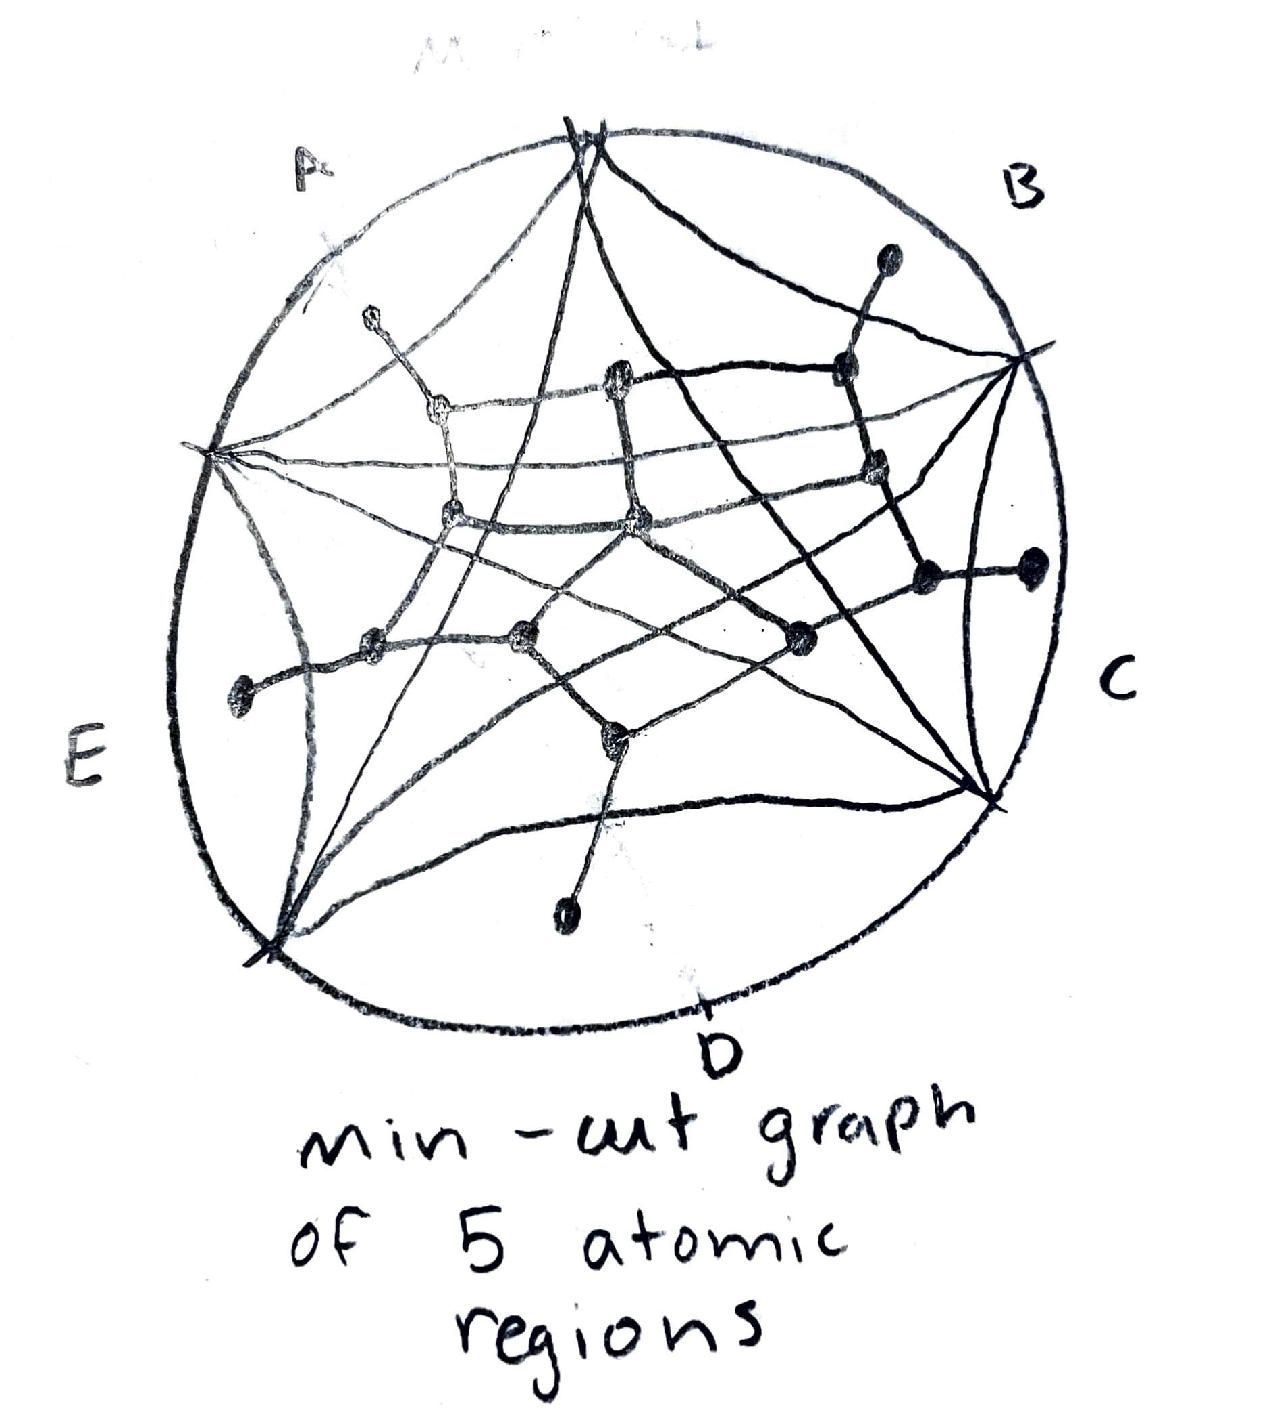
\includegraphics[width=0.8\textwidth]{min_cut_graph.pdf}
\end{center}

\subsection*{Official Statement}
Given as input a list of atomic boundary regions labeled \( 1, \dots, N \), a list of subsets of the regions \( R_1, \dots, R_k \subseteq [N] \), and a real-valued entropy \( S(R_i) \geq 0 \) for each \( R_i \), the weight of the minimum cut separating \( R_i \) from the rest of the boundary vertices (i.e., from \( [N] - R_i \)) is equal to \( S(R_i) \).

\subsection*{General Idea}
If we are given the complete entanglement structure of the boundary, we are therefore provided with a min-cut graph of the boundary entropies. We can then perform an experiment in the bulk space and use min-cut theory on the boundary to reconstruct the entropy graph. Giving us an interpretation of what the outcome would be in the bulk, because the boundary information is encoded in the bulk.

\textbf{This is basically the inverse min-cut problem.} Now we are given min-cut, find graph that gave you min-cut solution, therefore this graph is not unique. While the graph is not unique you can add on additional properties. For example, planar, few vertices. For this problem assume no wormholes. For DBRP to work we need to make ensure all quantum states satisfies properties (more on that later). \\
It is important to note and prove DBRP is computable, meaning it has an upper bound. \\
It has an upper bound of $2^{2^N}$

\section*{Proof:}
Given $K\leq2^N$ boundary regions form all $\leq2^N$ possible intersections of RT regions. At most 1 vertex needed in each region. Using linear programs for each edge weight takes "only" exp(exp(exp(N))) time!

\begin{center}
    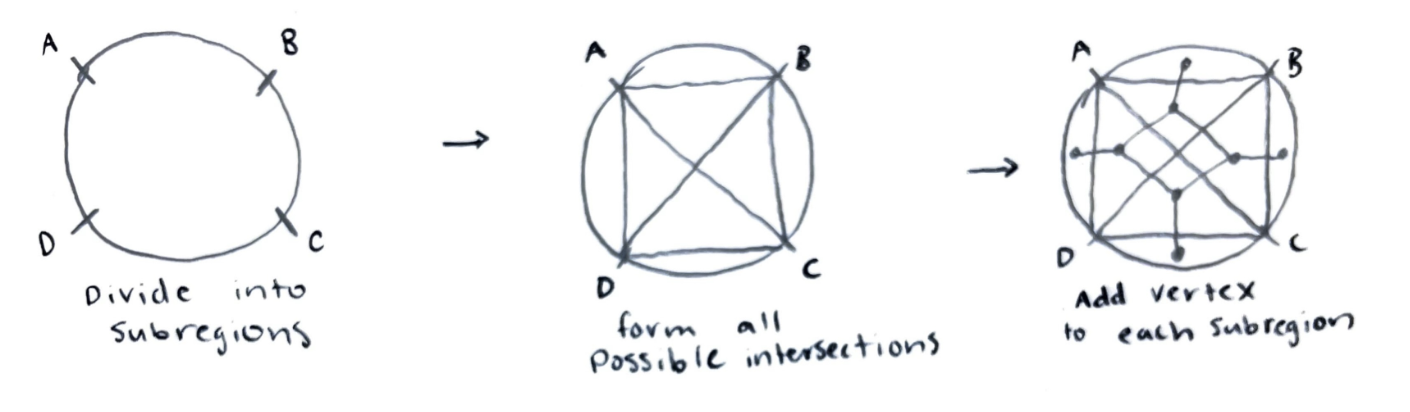
\includegraphics[width=0.8\textwidth]{subregions.png}
\end{center}

\subsection*{How to determine edge weights?}
Use linear programming, for every possibility of what min-cuts could be try to solve some linear equations and equalities. Can we set edge weights so that it will be min-cut?
\\Therefore, gives us algo for deciding any instance of DBRP.

\section*{Required Properties}
To ensure a solution exists we \textbf{need} the following properties:

\begin{enumerate}
    \item \textbf{Subadditivity (SA)}: entropy of \( A \) plus entropy of \( B \) is \( \geq \) entropy of \( A \cup B \)
    \[
    S(A) + S(B) \geq S(AB)
    \]
    \begin{center}
        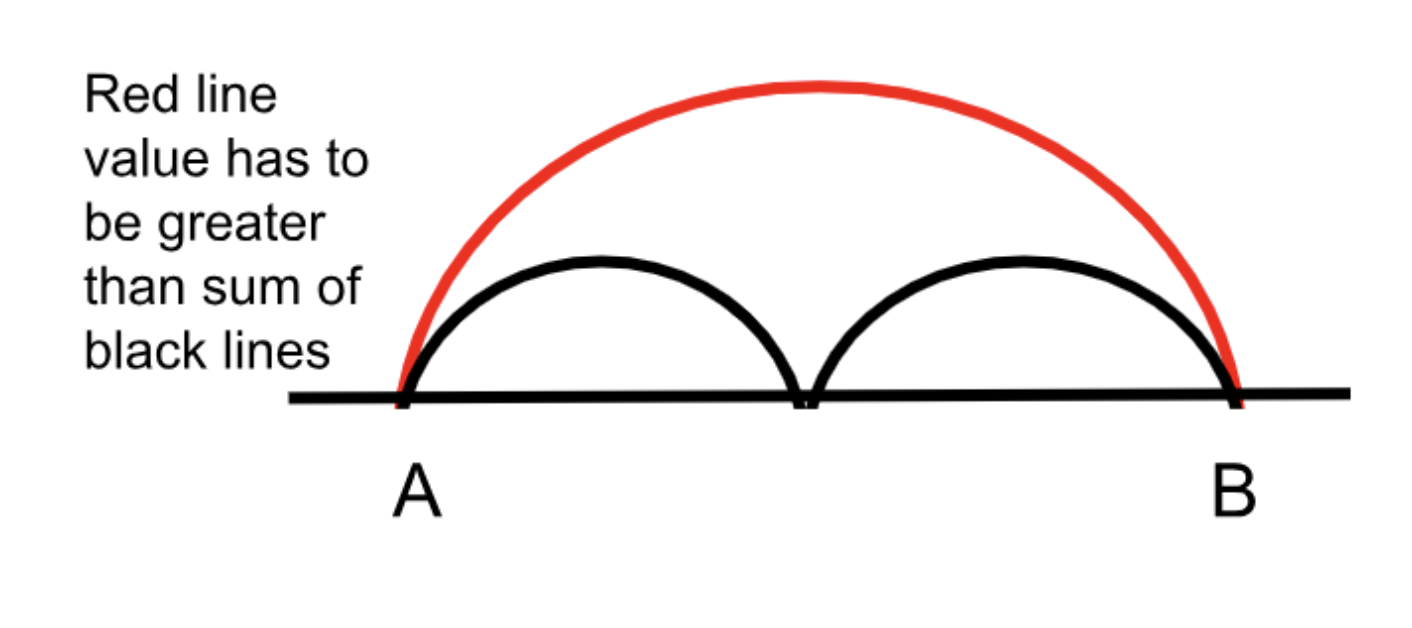
\includegraphics[width=\linewidth]{subaddivity.png}
    \end{center}
    
    \item \textbf{Strong Subadditivity (SSA)}
    \[
    S(AB) + S(BC) \geq S(B) + S(ABC)
    \]
    \begin{center}
        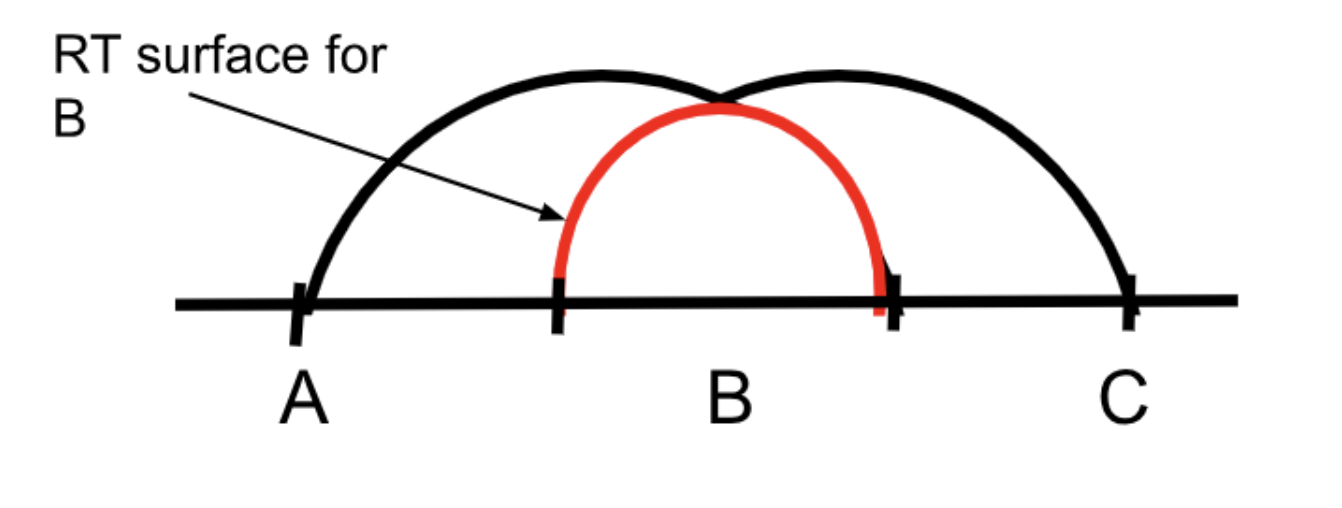
\includegraphics[width=0.8\textwidth]{strong_subaddivity.png}
    \end{center}
\end{enumerate}

\section*{Holographic Quantum State}
\begin{itemize}
    \item Boundary state in CFT that, due to holography, has a corresponding interpretation in bulk AdS space.
    \item This allows us to perform computations on a lower-dimensional boundary with no gravity, which then gives us information about higher-dimensional gravity in bulk space.
    \item Note: Entanglement entropy of a region in boundary can correspond to the area of the minimal surface in the bulk (RT-formula).
\end{itemize}

All holographic quantum states \textbf{must} satisfy the following property:
\begin{enumerate}
    \item \textbf{Monogamy of Mutual Information (MMI)}
    \[
    S(AB) + S(BC) + S(AC) \geq S(A) + S(B) + S(C) + S(ABC)
    \]
\end{enumerate}

\textbf{Question:} Are these properties what give us geometry?

\section*{DBRP on 1-dimensional Hilbert Space}
\begin{itemize}
    \item Note: To perform DBRP on a higher-dimensional Hilbert space, take the tensor product of each Hilbert space to create one large Hilbert space.
    \[
    \mathcal{H}_{\text{total}} = \mathcal{H}_1 \otimes \mathcal{H}_2 \otimes \dots \otimes \mathcal{H}_N
    \]
\end{itemize}
\begin{enumerate}
    \item Upper bound for contiguous boundary regions: 
    \[
    \frac{N(N-1)}{2}
    \]
    \item Can specify \textit{all} \( 2^N \) non-contiguous entropies in terms of \( \frac{N(N-1)}{2} \) contiguous entropies.
    \item Formula is minimum of 2 different possibilities:
    \[
    S(AC) = \min\{ S(A) + S(C), S(B) + S(D) \}
    \]
    \begin{figure}[htbp]  % 'h' places the figure "here" (can be adjusted)
        \centering
        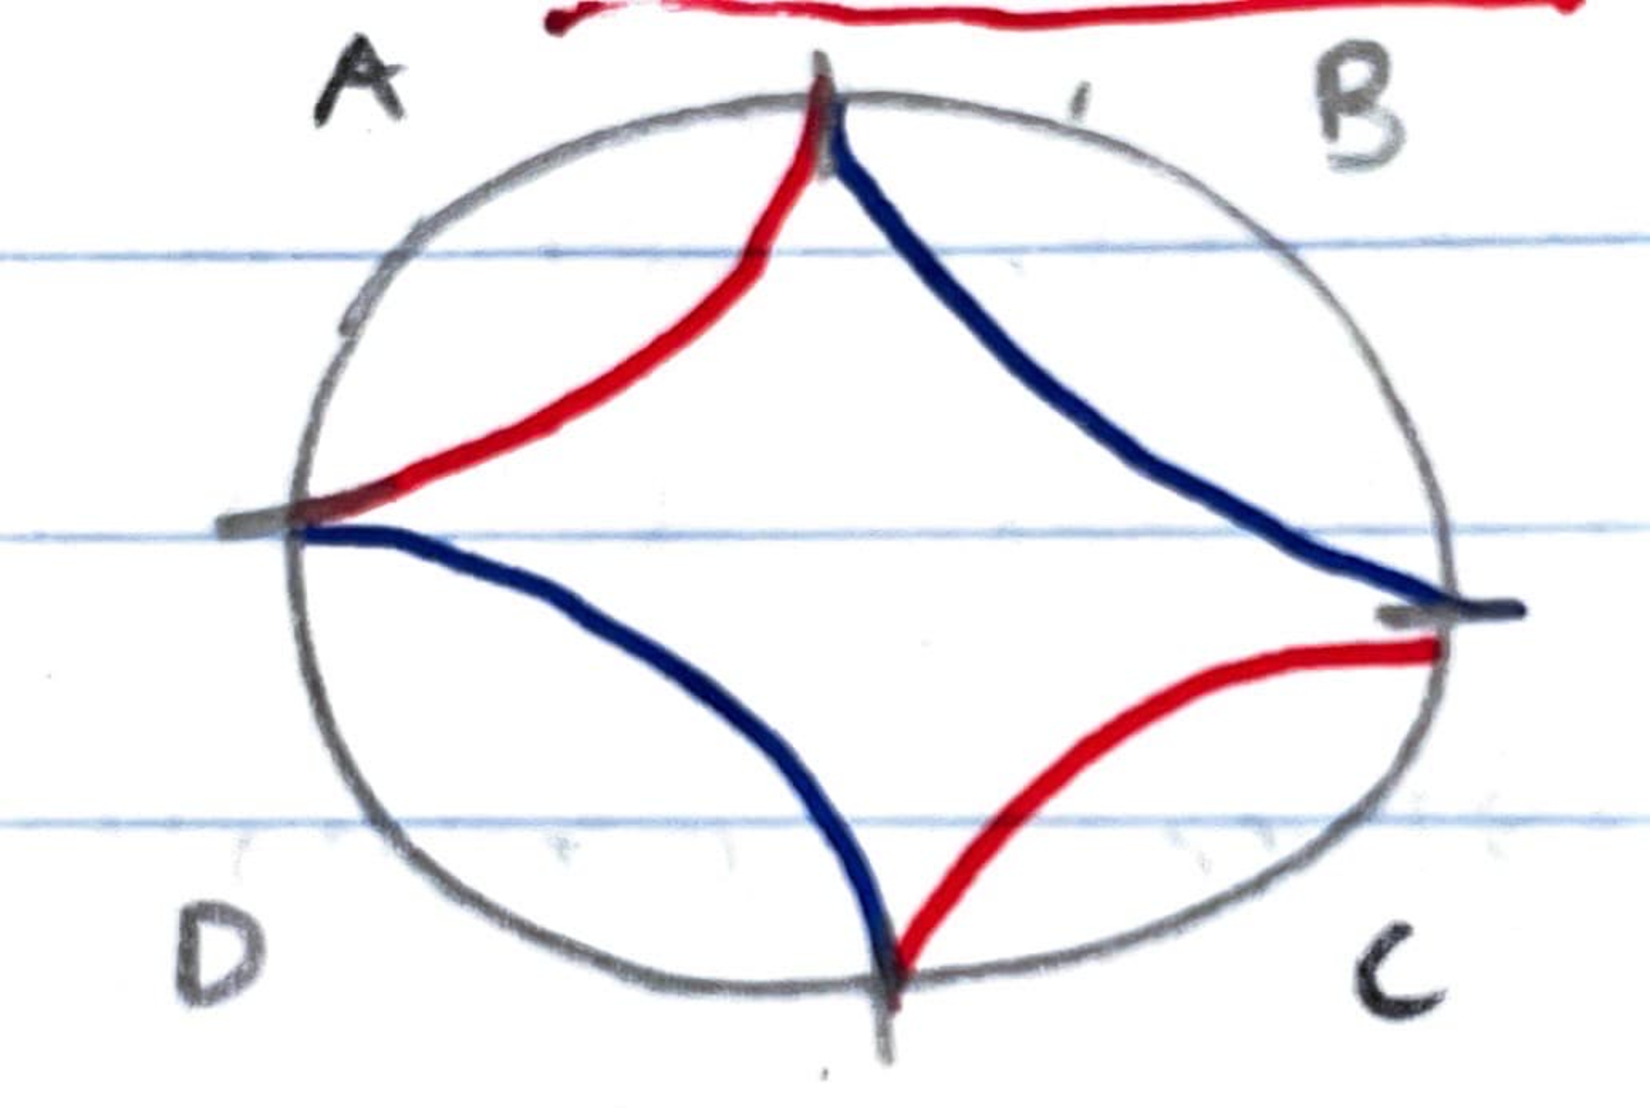
\includegraphics[width=0.8\textwidth]{parts.pdf}  % Adjust width as needed
        \caption{Where the first option is in red and second option is in blue}  % Caption text
        \label{fig:example}  % Label for referencing
    \end{figure}
\end{enumerate}


\section*{Theorem: 1D Boundary}
In special cases of a 1D boundary divided into \( N \) parts, given contiguous entropies satisfying SSA, we can always find a graph model of the bulk in linear time \( O(N^2) \). The graph model is planar, universal, and has \textbf{only} \( O(N^2) \) vertices.

\textbf{Note:} Only need to satisfy SSA for 1D.

\section*{Proof of 1D, with Examples}
\begin{itemize}
    \item Any contiguous boundary data that satisfies SSA admits a "bulkless" graph.
    \item A bulkless graph is a graph of pure edges and no vertices.
    \item After creating a bulkless graph, we can solve for what the edge weights should be! By using a system of linear equations, SSA ensures nonnegativity.
\end{itemize}


\begin{center}
    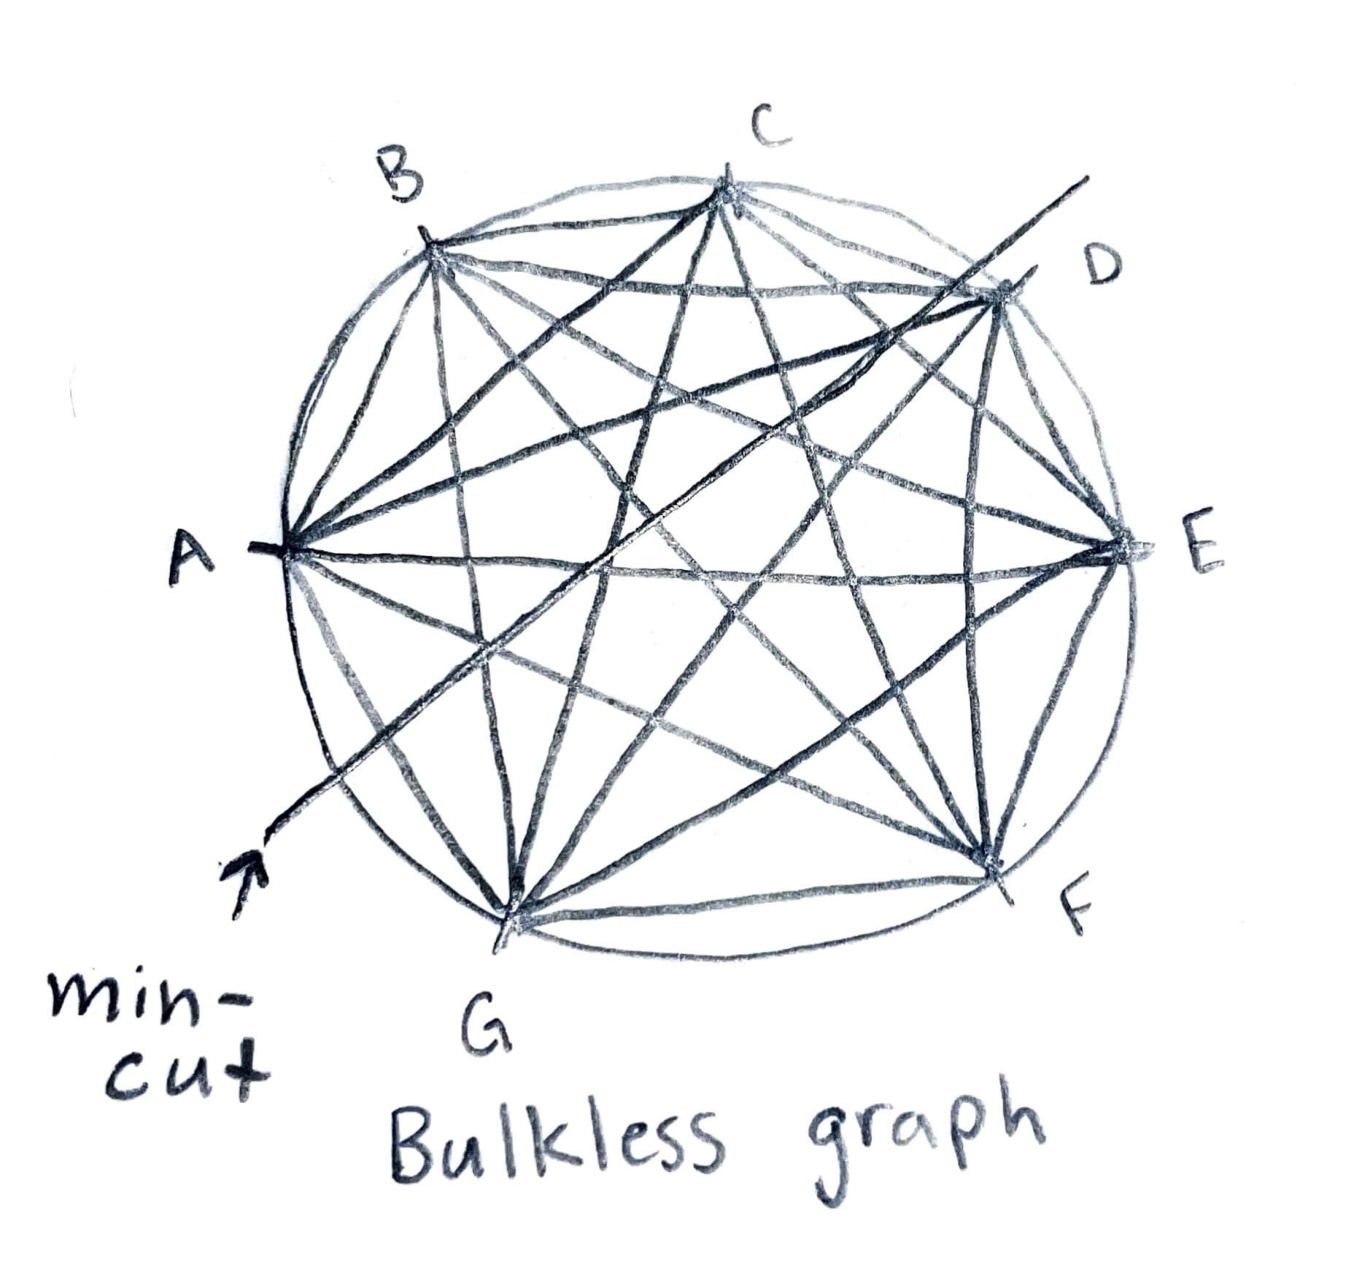
\includegraphics[width=0.6\textwidth]{bulkless_graph.pdf}
\end{center}

This will lead to a planar graph model of the bulk. The next step will be to get the model...

\section*{Chord Construction}
\begin{itemize}
    \item Get model of graph.
    \item Take all edges in between atomic boundary regions and add a chord (vertex) where each edge intersects.
    \item Edge weights = weights from bulkless graph.
\end{itemize}


\begin{center}
    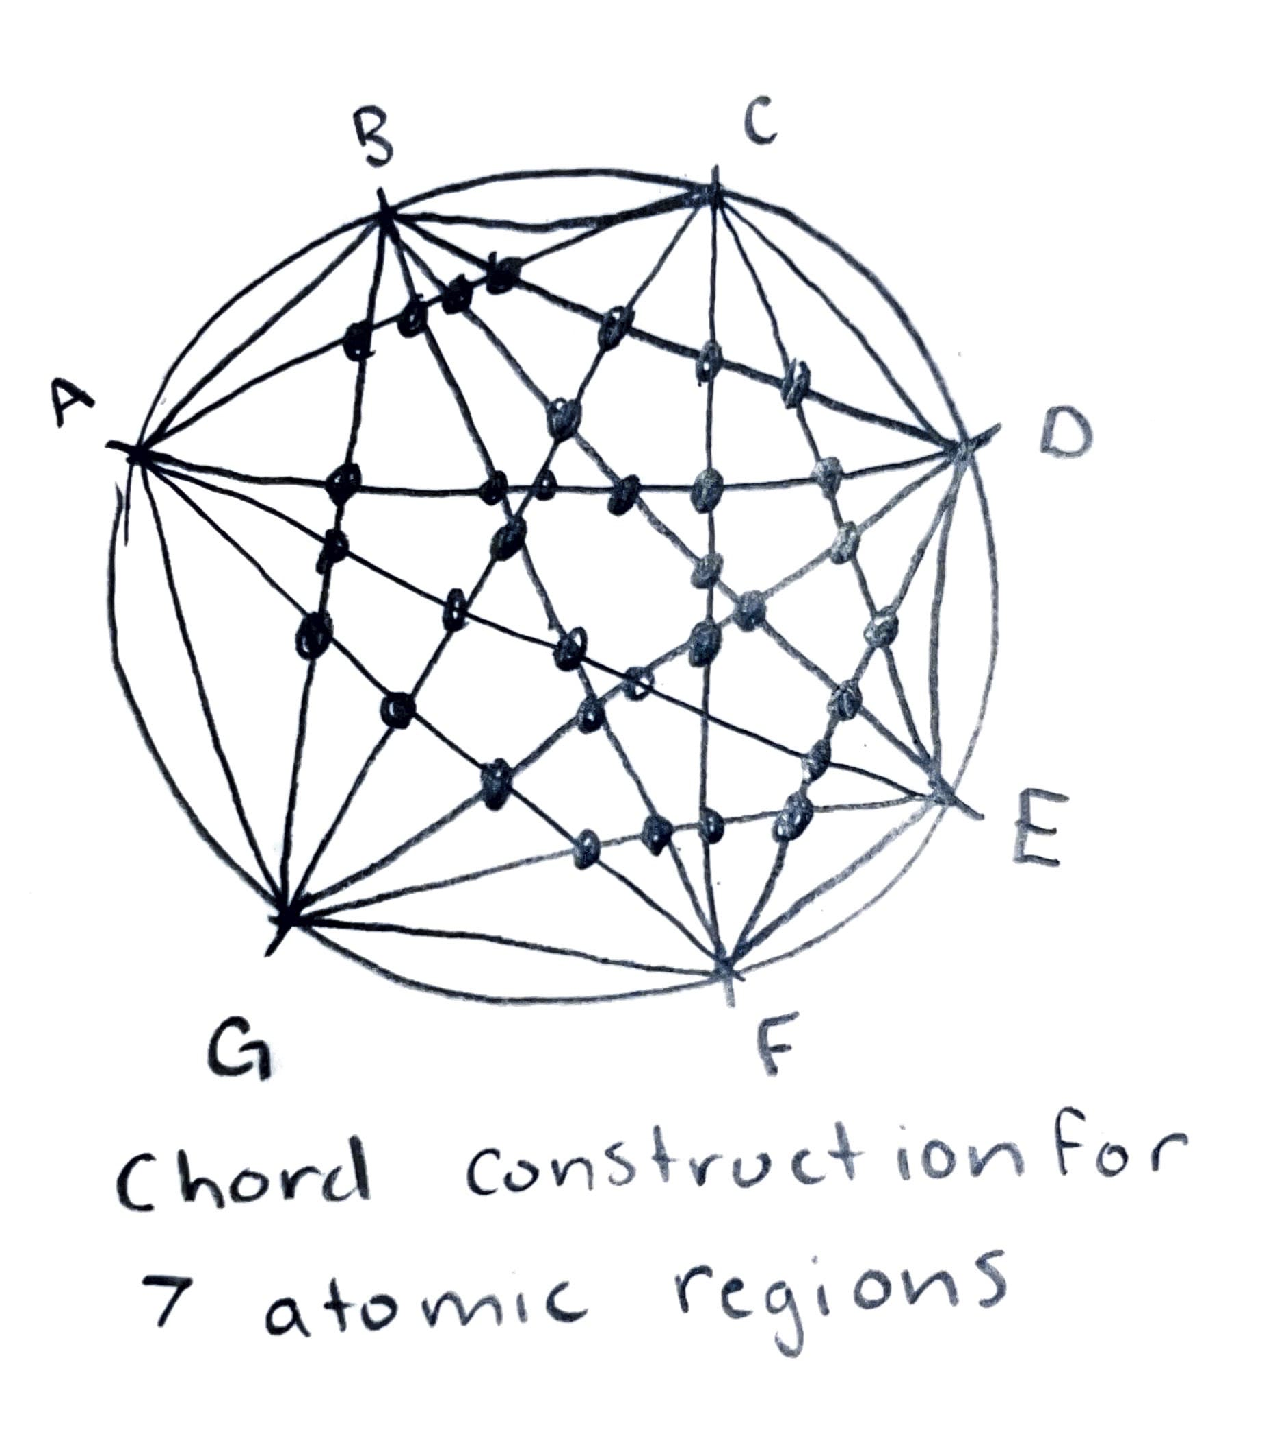
\includegraphics[width=0.6\textwidth]{chord_construct.pdf}
\end{center}

This yields a planar graph with \( O(N^4) \) vertices (not optimal) and the same cut structure as the bulkless graph.

\textbf{Note:} Since the bulkless graph has correct cut values, the planar graph will also have correct cut values. However, \( O(N^4) \) is not optimal, so a better construction was developed...

\section*{Diamondwork Construction}
\begin{itemize}
    \item Yields \( O(N^2) \) vertices and edges.
    \item Reduce via a planar graph made up of "overlapping" triangles, each contributing weight from the bulkless graph.
    \item Overlapping triangles are minimal surfaces that cut deeper into the bulk.
    \item Add edge weights together to overlap them.
    \item Min-cuts cut the same as the bulkless graph.
\end{itemize}

\begin{center}
    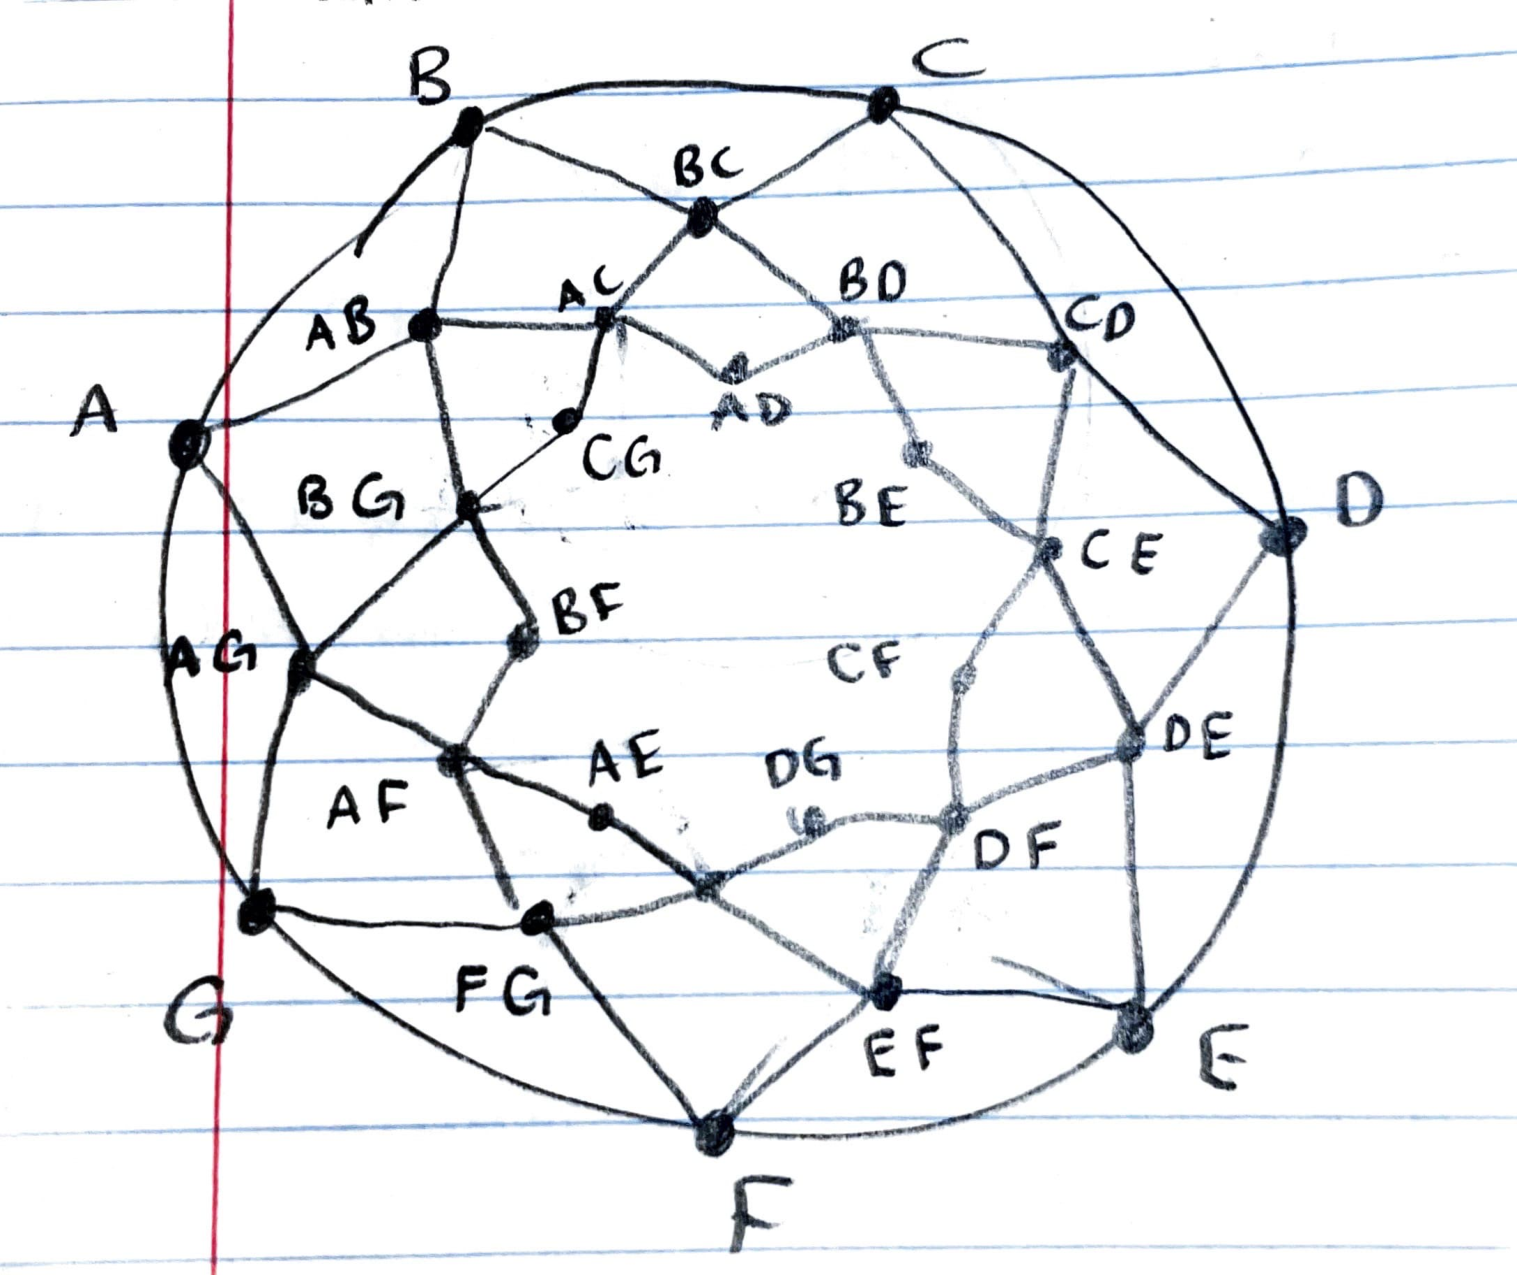
\includegraphics[width=0.6\textwidth]{edge_weights.pdf}
\end{center}

\section*{Harmonic Edge Weights}
This is the discrete version of AdS geometry. The entropy of a length \( L \) boundary region (where \( L \leq N/2 \)) is given as:

\begin{center}
    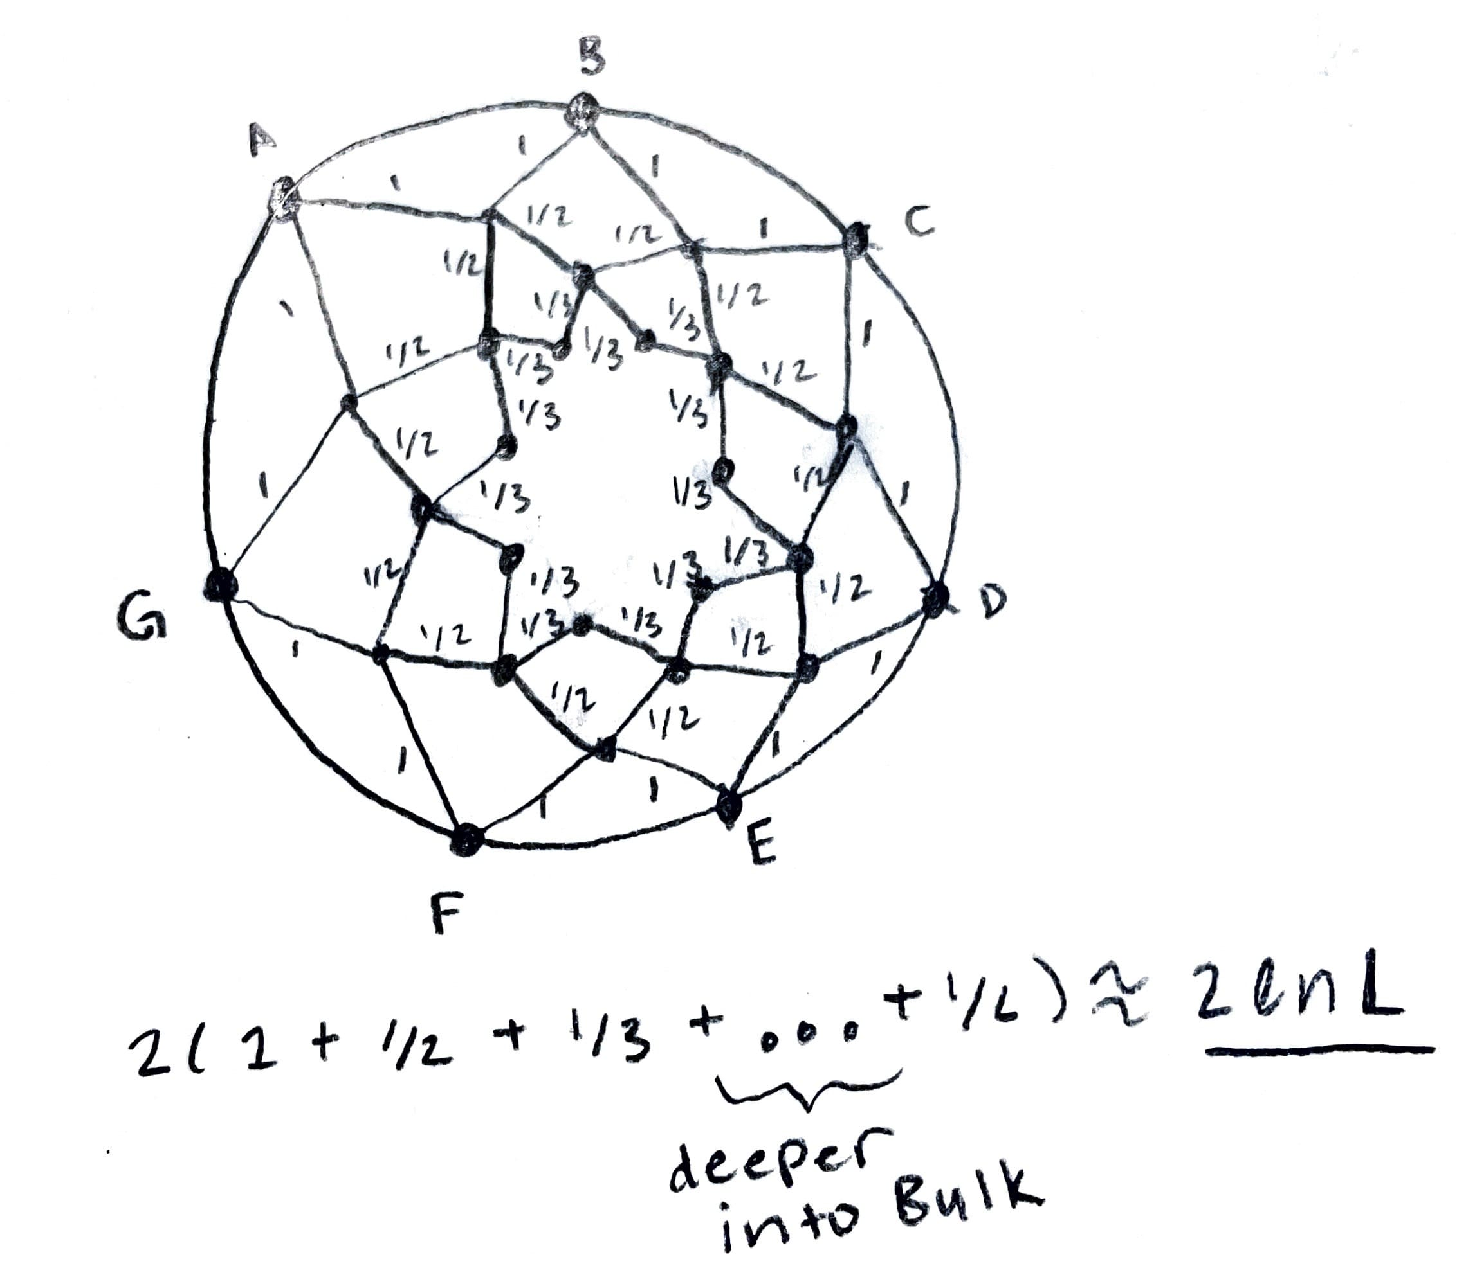
\includegraphics[width=0.8\textwidth]{harmonic.pdf}
\end{center}

\section*{Why No Black Holes?}
\begin{itemize}
    \item All edge weights have the same value, therefore the RT minimal surface means nothing.
    \item There is no advantage to cutting deeper into the bulk.
\end{itemize}

\begin{center}
    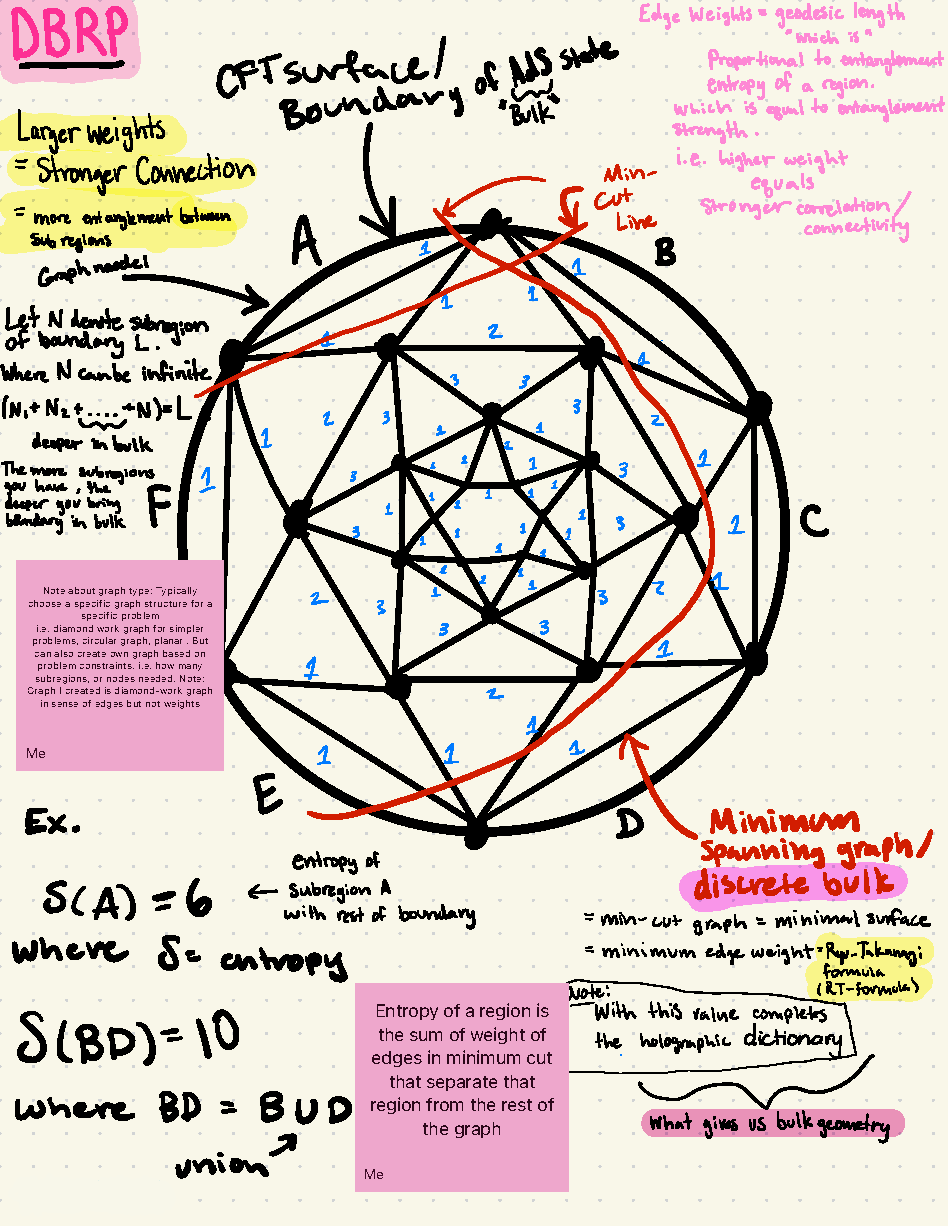
\includegraphics[width=0.8\textwidth]{dbrp_summed.pdf}
\end{center}

\section{Conclusion}
Summarize key findings, limitations, and possible future research directions

\newpage

%%%%%%%%%%%%%%%%%%%%% REFERENCES %%%%%%%%%%%%%%%%%%%%%%%
\begin{thebibliography}{9}
    \bibitem{example}
    Scott Aaronson and Jason Pollack, \textit{Discrete bulk reconstruction}, 2023.
    \bibitem{2}
    Ronak Ramachandran, \textit{Further Exploration of the Discrete Bulk Reconstruction Problem}, 2023.
    \bibitem{AI}
    ChatGPT
\end{thebibliography}

\end{document}

